\documentclass[12pt]{article}
\usepackage{fullpage}
\usepackage{url}
\usepackage{amsmath}
\usepackage{amsfonts}
\usepackage{algorithm}
\usepackage{algorithmic}
\usepackage{graphicx}
\usepackage{hyperref}
\usepackage{color}
\usepackage{listings}
\usepackage{verbatim}
\usepackage{enumitem}
\usepackage[parfill]{parskip}

\newcommand{\xb}{\mathbf{x}}
\newcommand{\yb}{\mathbf{y}}
\newcommand{\wb}{\mathbf{w}}
\newcommand{\Xb}{\mathbf{X}}
\newcommand{\Yb}{\mathbf{Y}}
\newcommand{\tr}{^T}
\newcommand{\hb}{\mathbf{h}}
\newcommand{\Hb}{\mathbf{H}}

\newcommand{\cmt}[1]{{\footnotesize\textcolor{red}{#1}}}
\newcommand{\todo}[1]{\cmt{TO-DO: #1}}

\title{CS294-112 Deep Reinforcement Learning HW4}

\author{ Heri Zhao
}

\date{Fall 2018}

\usepackage{courier}
 
\definecolor{codegreen}{rgb}{0,0.6,0}
\definecolor{codegray}{rgb}{0.5,0.5,0.5}
\definecolor{codepurple}{rgb}{0.58,0,0.82}
\definecolor{backcolour}{rgb}{0.95,0.95,0.92}

\lstdefinestyle{mystyle}{
    backgroundcolor=\color{backcolour},   
    commentstyle=\color{codegreen},
    keywordstyle=\color{magenta},
    numberstyle=\tiny\color{codegray},
    stringstyle=\color{codepurple},
    basicstyle=\footnotesize\ttfamily,
    breakatwhitespace=false,         
    breaklines=true,                 
    captionpos=b,                    
    keepspaces=true,                 
    %numbers=left,                    
    numbersep=5pt,                  
    showspaces=false,                
    showstringspaces=false,
    showtabs=false,                  
    tabsize=2
}

\lstset{style=mystyle}

\begin{document}

\maketitle

\section*{Problem 1}

\subsection*{(a)}
\begin{figure}[H]
  \centering
  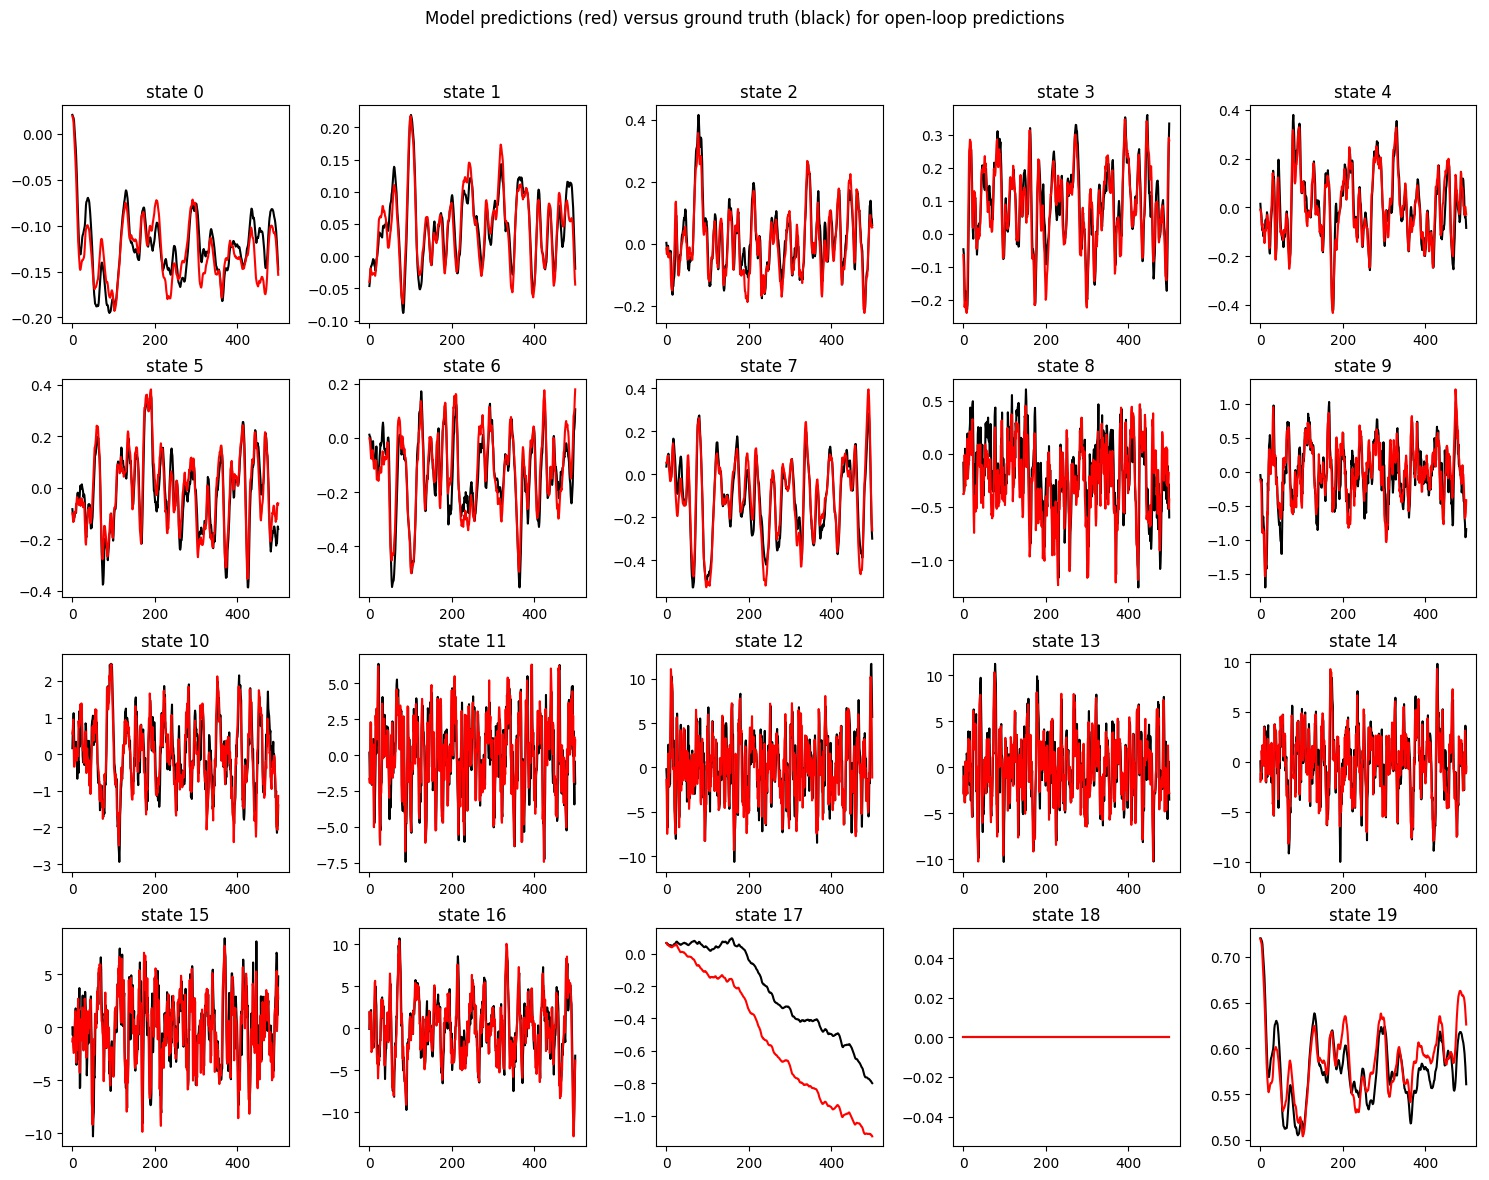
\includegraphics[height=3.4in]{prediction_001.jpg}
  \caption{Mostly accurate dynamics model predictions}
\end{figure}

\subsection*{(b)}
State 17 is the most inaccurate prediction. This is the distribution mismatch problem since we have fixed dataset here. Intuitively, the earlier prediction error will accumulate and we finally end up with large prediction error.

\newpage
\section*{Problem 2}
\begin{table}[H]
\begin{center}
  \begin{tabular}{ c | c | c }
    \hline
    & Random policy & Model-based policy \\ \hline
    ReturnAvg & -152.333 & 29.7827 \\ \hline
    ReturnStd & 29.1592 & 29.6192 \\ \hline
  \end{tabular}
  \caption{ReturnAvg \& ReturnStd for random policy and model-based policy}
\end{center}
\end{table}


\newpage
\section*{Problem 3a}
\begin{figure}[H]
  \centering
  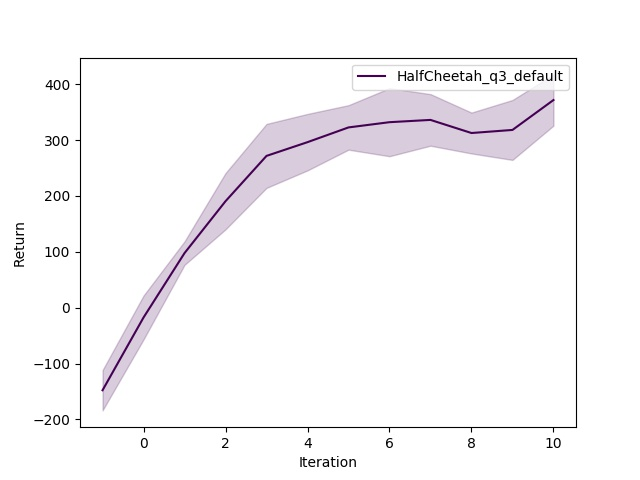
\includegraphics[height=3.4in]{HalfCheetah_q3_default.jpg}
  \caption{Returns versus iteration for default setting}
\end{figure}

\newpage
\section*{Problem 3b}

\subsection*{(a)}
\begin{figure}[H]
  \centering
  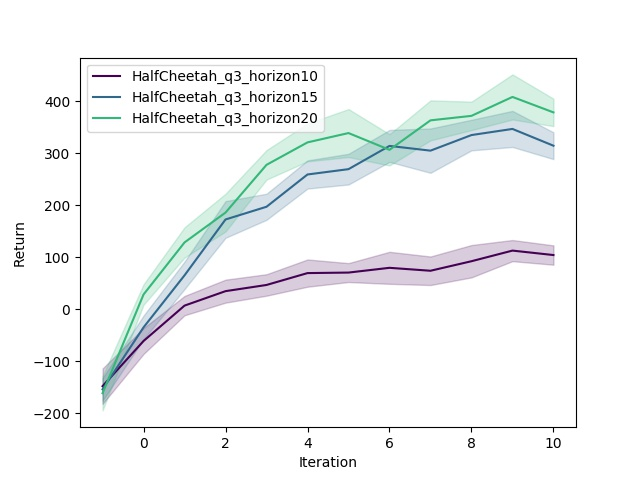
\includegraphics[height=3.4in]{HalfCheetah_q3_mpc_horizon.jpg}
  \caption{Comparison performance when varying the MPC horizon}
\end{figure}
We can see that the higher horizon for the policy the better performance it generates. This makes sense intuitively since if the policy could plan further in the future, it should perform better.

\subsection*{(b)}
\begin{figure}[H]
  \centering
  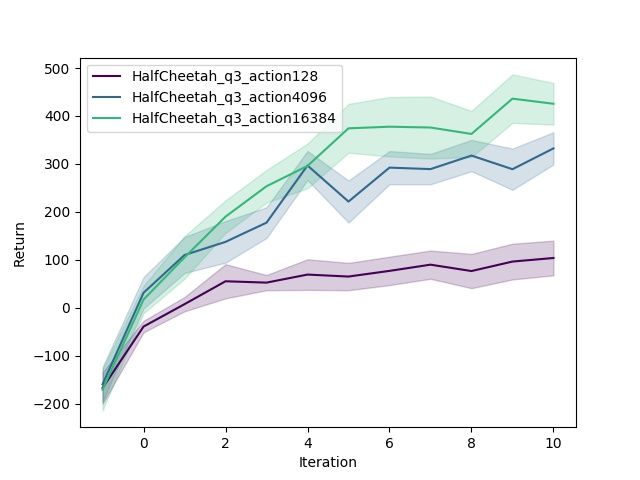
\includegraphics[height=3.4in]{HalfCheetah_q3_actions.jpg}
  \caption{Comparison performance when varying the number of randomly sampled action sequences used for planning}
\end{figure}
We can see that the more actions we sampled, the better performance the policy generates, since by sampling more trajectories, we have larger chances to get optimal action.


\subsection*{(c)}
\begin{figure}[H]
  \centering
  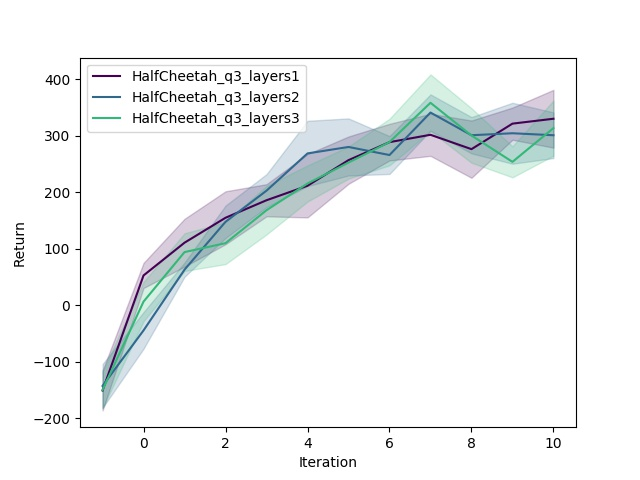
\includegraphics[height=3.4in]{HalfCheetah_q3_nn_layers.jpg}
  \caption{Comparison performance when varying the number of neural network layers for the learned dynamics model}
\end{figure}
There was a bug in the code... and that's why they are almost the same. The guess would be that the more layers we have, the better performance we should be able to get.

\newpage
\section*{Bonus - CEM}
\begin{figure}[H]
  \centering
  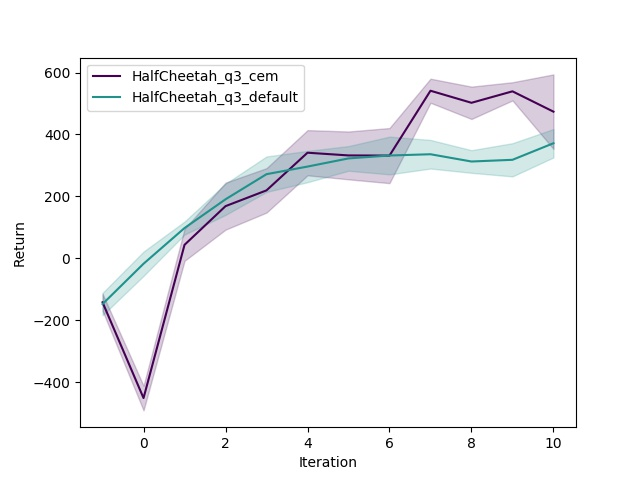
\includegraphics[height=3.4in]{HalfCheetah_q3_bonus.jpg}
  \caption{Comparison performance CEM vs uniform random action selection}
\end{figure}
We can see that at the beginning, the return dropped a lot, this might be caused by our distribution initialization. Later on, the performance increased a lot to around 600 compared with the default 300-350. I think the performance could be better if we tune the parameter \textit{maxits} and \textit{Ne}. \\

For implementation, please check \textbf{\_setup\_action\_selection\_cem(self, state\_ph)} in \\
model\_based\_policy.py.

To run:
\begin{lstlisting}[language=bash]
python main.py q3 --cem
\end{lstlisting}

\end{document}













